\documentclass[12pt]{report}

\usepackage[a4paper,width=150mm,top=25mm,bottom=25mm,bindingoffset=6mm]{geometry}
\usepackage[onehalfspacing]{setspace}
\usepackage{ucs}
\usepackage[table,xcdraw]{xcolor}
\definecolor{mColor1}{rgb}{0.9,0.9,0.9}

\usepackage{fancyhdr}
\pagestyle{fancy}
\fancyhead{}
\renewcommand{\chaptermark}[1]{\markboth{#1}{}}
\renewcommand\sectionmark[1]{\markright{\thesection\ #1}}

\fancyhead[LO, RE]{\leftmark}
\fancyhead[LE, RO]{\rightmark}

\usepackage{titlesec, blindtext, color}
\definecolor{gray75}{gray}{0.75}
\usepackage{mathptmx}
\usepackage[utf8]{inputenc}
\usepackage[T1]{fontenc}
\usepackage[ngerman]{babel}

\usepackage{amsmath,amssymb,amstext,amsthm,mathtools}
\usepackage{url}
\usepackage{caption}
%\usepackage[belowskip=-5pt,aboveskip=0pt]{caption}
\usepackage{subcaption}

\usepackage{float}
\usepackage{lscape}
\usepackage{pdfpages}
\usepackage{rotating}
\usepackage{graphicx}
\setlength\parindent{0pt}
\usepackage{hyperref}
\usepackage{acronym}
\usepackage{textcmds}
\usepackage{longtable}
\usepackage[export]{adjustbox}
\usepackage{upgreek}
\usepackage{dsfont}
\usepackage{tensor}
\usepackage{amsbsy}
\usepackage{multirow, hhline, colortbl}
\usepackage[table]{xcolor}


\DeclareMathAlphabet{\mathcal}{OMS}{cmsy}{m}{n}
\SetMathAlphabet{\mathcal}{bold}{OMS}{cmsy}{b}{n}

\usepackage{listings, lstautogobble}
\usepackage{textcomp}
\definecolor{yo}{rgb}{0.9,0.6,0}
\definecolor{Gray}{gray}{0.9}
\definecolor{listinggray}{gray}{0.9}
\definecolor{lbcolor}{rgb}{0.95,0.95,0.95}
\definecolor{greylines}{rgb}{0.9529,0.9529,0.9529}

\lstset{
	backgroundcolor=\color{lbcolor},
	tabsize=4,
	rulecolor=,
	language=python,
        basicstyle=\scriptsize,
        upquote=true,
        aboveskip={1.5\baselineskip},
        columns=fixed,
        showstringspaces=false,
        extendedchars=true,
        breaklines=true,
        prebreak = \raisebox{0ex}[0ex][0ex]{\ensuremath{\hookleftarrow}},
        frame=lines,
        showtabs=false,
        showspaces=false,
        showstringspaces=false,
        identifierstyle=\ttfamily,
        keywordstyle=\color[rgb]{0.55,0,0},
        alsoletter={/,*,[,]},%
        otherkeywords={},
        morekeywords=[2]{with, as},
        morekeywords=[3]{},
        emph={self},          % Custom highlighting
		emphstyle=\color[rgb]{0.1,0.3,1},
		emph={[2]f},          % Custom highlighting
		emphstyle={[2]\color[rgb]{0.1,0.5,0.1}},
		emph={[3]__init__},          % Custom highlighting
		emphstyle={[3]\color[rgb]{0.1,0.3,1}},
		emph={[4]open,str,print,KeyError},          % Custom highlighting
		emphstyle={[4]\color[rgb]{0.2,0.6,0.8}},
        commentstyle=\color[rgb]{0.3,0.3,0.3},
        stringstyle=\color[rgb]{0.133,0.545,0.133},
        	autogobble=true
}
\lstnewenvironment{ttlisting}{\lstset{basicstyle=\scriptsize}}{}

\usepackage{color}
\usepackage[section]{placeins}

\newenvironment{simplechar}{%
	\catcode`\$=12
	\catcode`\&=12
	\catcode`\#=12
	\catcode`\^=12
	\catcode`\_=12
	\catcode`\~=12
	\catcode`\%=12
	\catcode`\"=12
	\catcode`\'=12
	}{}{}

\newtheoremstyle{dotless}{}{}{\itshape}{}{\bfseries}{}{ }{}

\theoremstyle{dotless}

\newtheorem{thm}{Theorem}
\newtheorem{defn}[thm]{Definition}
\newtheorem{exmp}[thm]{Example}
\theoremstyle{definition}


\begin{document}

\begin{titlepage}
	Warum bin ich nicht einfach Staubsaugervertreter geworden?
\end{titlepage}

\tableofcontents


\chapter{Grundlagen interner Modelle im Kompositbereich}

\subsubsection{Definition eines Unternehmensmodell}
Bei einem internen Risikomodell handelt es sich um ein stochastisches Modell, das mittels stochastischer Verfahren messbare Aktiv- und Passivrisiken der betrachteten Gesellschaften abbildet. \\
Dabei sollte es über die unternehmensindividuelle Modellierung der stochastischen Geschäftsgrößen die signikanten finanziellen Auswirkungen konsistent quantifizieren und Abhängigkeitsstrukturen zwischen alle Risikogrößen berücksichtigen.\\
Zielgrößen sind die Gesamtverteilung der Geschäftsergebnisse sowie die Berechnung des benötigten Risikokapitals in einer Marktwertsicht (Anfalljahressicht).

\subsubsection{Standardformel}
\begin{itemize}
\item Anwendung vorgegebener Stressparameter / Risikofaktoren / Szenarien pro Einzelmodul (jeweils kalibriert auf den 200-Jahresstress) ergibt Einzel-SCR
\item Jeweils Ein-Punkt-Betrachtung aller Risiken (Value-at-Risk Ansatz)
\item Anschließende Aggregation der Einzel-SCRs mit der Wurzelformel anhand von vorgegebenen Korrelationsparametern.
\end{itemize}

\subsubsection{Modellierung mit einem stochastischen Unternehmensmodell}

\begin{figure}[ht]
	\centering
	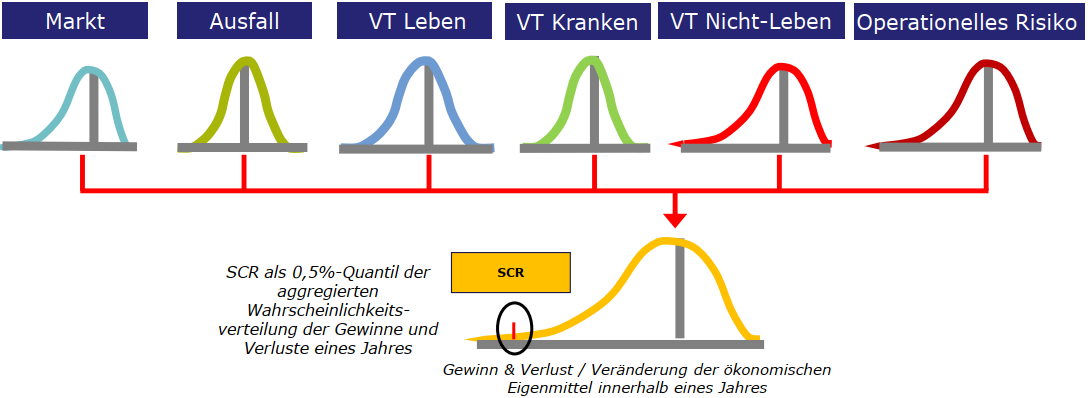
\includegraphics[width= 0.7\textwidth]{Bilder/StochUnternehmensmodell.png}
\end{figure}

\begin{itemize}
\item Simulationsbasiert: Hohe Anzahl an Simulationen erforderlich
\item separate komplette Wahrscheinlichkeitsverteilung per Risiko (jedes Risiko wird durch eine stochastische Ergebnisgröße repräsentiert
\item Segmentierung und Kalibrierung (Verteilungen, Volatilitätsparameter) erfolgt unternehmensindividuell, Aggregation unter Copula-Annahmenil
\item Beliebige Risikomaße anwendbar - neben VaR auch Expected Shortfall
\end{itemize}


\subsubsection{Definitionen}
Ausgangspunkt: Gegeben seien $n \in \mathbb{N}$ Simulationswerte $(^{(1)}X, ^{(2)}X, ..., ^{(n)}X)$ einer Verlustvariable $X$ sowie das Sicherheitsniveau $\alpha \in ]0;1[$. Weiterhin bezeichne $m:= \lfloor n \cdot (1- \alpha) \rfloor$ die Gaußklammer von $n \cdot (1- \alpha)$ und $(^{(1\downarrow n)}X, ^{(2\downarrow n)}X, ..., ^{(n\downarrow n)}X)$ die obere Ordnungsstatistik mit $^{(1\downarrow n)} X \geq ^{(2\downarrow n)} X \geq ... \geq ^{(n\downarrow n)} X$

\begin{figure}[ht]
	\centering
	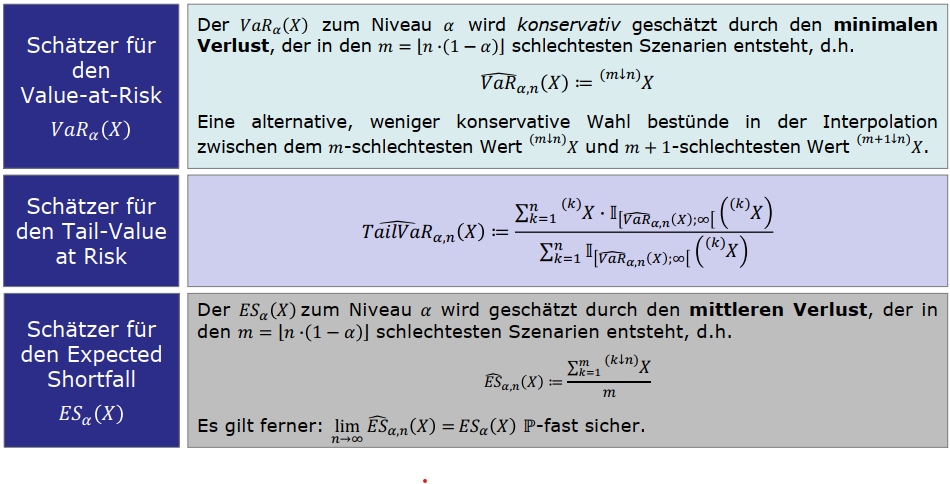
\includegraphics[width= \textwidth]{Bilder/Definitionen1.png}
\end{figure}

\subsubsection{Struktur eines DFA-Modells (Dynamische Finanzanalyse in S/U}

\begin{figure}[ht]
	\centering
	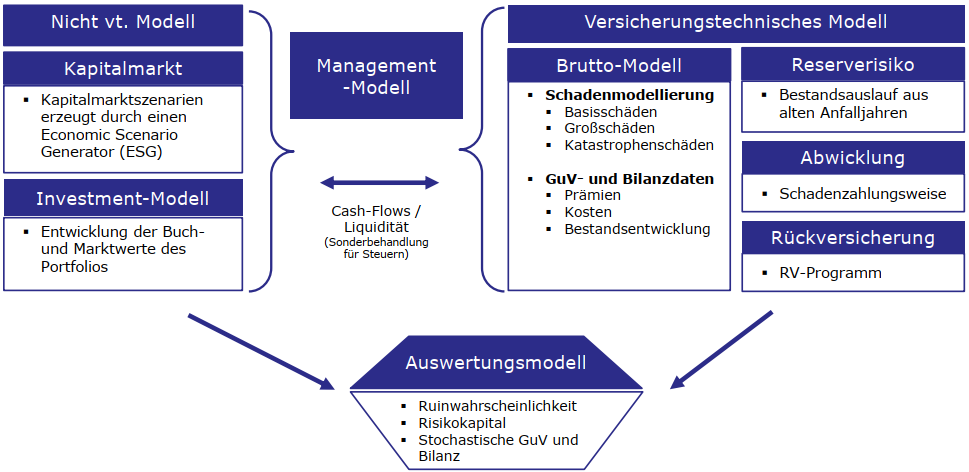
\includegraphics[width=\textwidth]{Bilder/DFA.png}
\end{figure}


\chapter{Bruttomodellierung (inkl. Katastrophenschäden)}

\section{Grundlagen}

\subsection{Zielgrößen und Gestalt der Ergebnisse}
Bei der Betrachtung des Versicherten-/ Schadenbestands lassen sich zwei Zeithorizonte bzw. Sichtweisen unterscheiden, die zu unterschiedlichen Risikodefinitionen führen:

\subsubsection{Kalenderjahressicht}

\begin{figure}[ht]
	\centering
	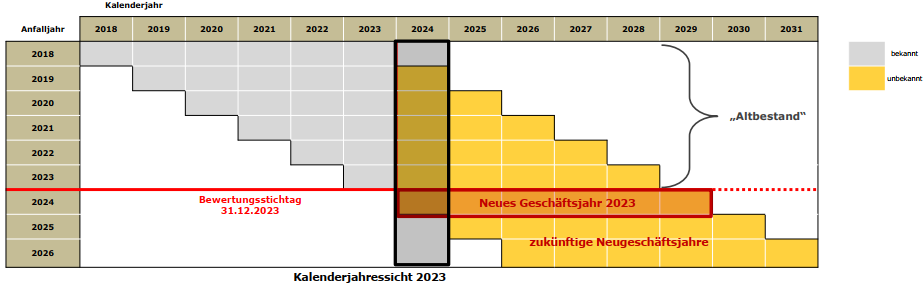
\includegraphics[width= \textwidth]{Bilder/Kalendersicht.png}
\end{figure}

\begin{itemize}
\item Neugeschäftsentwicklung im kommenden Kalenderjahr (Zahlungen + ausgehende Reserven)
\item Abwicklung des Altbestands im kommenden Kalenderjahr
\item Risikohorizont von Solvency II: Bemessungsgrundlage für die Wahrscheinlichkeit, innerhalb eines Kalenderjahres Ruin zu erleiden
\item Teilweise auch längere Zeithorizonte
\item Mögliche Verwendungszwecke: Berechnung des regulatorischen SCRs (bei internem Modell) bzw. Gesamtsolvabilitätsbedarf , Limitsysteme, Risikomarge für vt. Rückstellungen
\end{itemize}

\subsubsection{Ultimatesicht}

\begin{figure}[ht]
	\centering
	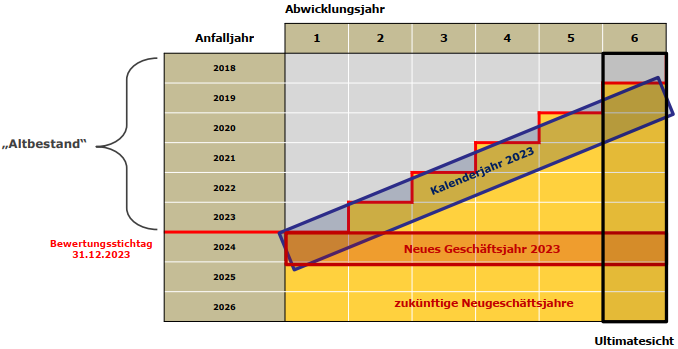
\includegraphics[width= \textwidth]{Bilder/Ultimatesicht.png}
\end{figure}

\begin{itemize}
\item Betrachtung der Ergebnisgrößen und damit verbundener Unsicherheiten über die komplette Abwicklungsdauer bis zum Endschadenstand = Ultimate auf einer Anfalljahresbasis
\item resultiert in "natürlicher" Betrachtung der vt. Risiken
\item entspricht nicht dem Risikohorizont, wie in SII für SCR vorgibt
\item Mögliche Verwendungszwecke: Profitatbilitäsmessung, Rückversicherungsanalyse, Risikozuschläge für Tarifierung
\end{itemize}

\subsection{Definition des Prämienrisikos}

Das Prämienrisiko
\begin{itemize}
\item resultiert aus der Unsicherheit / Volatilität in Bezug auf Prämien, Schaden und Kosten aus zukünftiger Risikotragung
\item bezieht sich somit nur auf diejenigen Schäden, die innerhalb des modellierten Neugeschäftsjahres (Anfalljahressicht) anfallen
\end{itemize}

Das ultimative Prämienrisiko (synonym: Zeichnungsrisiko) bezeichnet das Risiko,
dass die Prämien des Neugeschäftsjahres nicht ausreichen, um die zugehörigen Schäden
und Kosten bis zur vollständigen Abwicklung zu decken.

\subsubsection{Definition}
Das (nominale) Anfalljahresergebniss $T$ (= Technical Result) des Neugeschäftsjahres wird definiert als: $T:= P - E - U$, mit \\
P: verdiente Prämie des Neugeschäftsjahres nach vollständiger Abwicklung\\
E: Kosten des Neugeschäftsjahres nach vollständiger Abwicklung \\
U: Endschadenaufwand des Neugeschäftsjahres nach vollständiger Abwicklung \\

Das Anfalljahresergebnis $T$ ist eine Gewinnvariable: \\
$T>0$ ist äquivalent zu $P>E*U$ und bedeutet einen zukünftigen Gewinn \\
während $T<0 \Leftrightarrow P<E*U$ einen zukünftigen Verlust entspricht.

Alternative Defintion: ultimative Prämienrisiko (synonym: Zeichnungsrisiko) bezeichnet das Risiko, dass das Anfalljahresergebnis des Neugeschäftsjahres nach vollständiger Abwicklung negativ ist.

\subsubsection{Frage: Sollte man das ultimative Prämienrisiko anhand des Anfalljahresergebnisses vor oder nach Zentrierung, d.h. vor oder nach Abzug des Mittelwerts, messen?}
U.a. abhängig vom Verwendungszweck der Ergebnisse:
\begin{itemize}
\item Liegt Fokus auf Auswirkungen auf die Kapitalsituation?
\item Sind Erträge und Verluste aus zukünftigen Neugeschäft in Eigenmitteln enthalten?
\item Primär Darstellung Ergebnisvolatilität?
\item Weitere Überlegungen:
\begin{itemize}
\item Das erwartete Ergebnis (= Mittelwert der Simulationen) entspricht nicht zwingend dem geplantem Ergebnis
\item Bei hochprofitablem Geschäft ist ohne Zentrierung des originären Anfalljahresergebnisses bei bestimmten Risikomaßen (Bsp: VaR) sogar ein negatives Risikokapital möglich.
\end{itemize}
\end{itemize}

Ergebnisgrößen für das Prämienrisiko:
\begin{itemize}
\item Ergebniskomponenten:
\begin{itemize}
\item Verdiente Prämie: i.d.R. fix, bei mehrjähriger Projektion sit Prämienzyklus zu berücksichtigen
\item Kosten: getrennt nach Vertrieb, Regulierung und Verwaltung
\item Schäden: stochastische Modellierung, zwecks genauer Abbildung der Rückversicherungsstruktur und Modellierung der spartenspezifischen Schadenvolatilitätn erfolgt Trennung nach Schadentp (Einzelne Großschäden, Einzelne Ereignisse)
\end{itemize}
\item Segmentierung/ Modellierungstiefe: 
\begin{itemize}
\item Aufteilung in HUK und Sach
\item Bsp. HUK: Kasko, Haftpflicht, Unfal
\item Bsp. Sach: VGV, Feuerindustrie
\end{itemize}
\end{itemize}

\subsection{Schadenmodellierung}
Trennung der Schadentypen: Basisschäden, Großschäden, Katastrophenschäden

\subsubsection{Basisschäden}
\begin{itemize}
\item hohe Schadenfrequenz und geringe Schadenhöhe
\item Simulation als Aggregat
\item Parametrisierung auf Basis eigener Schadenerfahrung
\end{itemize}

\subsubsection{Großschäden}
\begin{itemize}
\item Schäden oberhalb spezifischen Schwellenwerts
\item geringe Frequenz, große Schadenhöhe
\item Modellierung: Einzelbasis nach dem kollektiven Modell
\item Parametrisierung auf Basis eigener Schadenerfahrung
\end{itemize}

\subsubsection{Katastrophenschäden}
\begin{itemize}
\item sehr niedrige Eintrittswahrscheinlichkeit, extreme Schadenhöhe
\item Trennung nach Naturgefahren, Man-Made Gefahren, sonstiges wie Pandemien
\item Charakteristika Naturgefahren: Treffen größere Region, Ereignisschaden setzt sich aus vielen kleinen Einzelschäden zusammen, Schäden betreffen viele Sparten gleichzeitig (Wohngebäude, Hausrat, Kraftfahrt...)
\item Charakteristika Man-Made Gefahren: hohes Schadenpotenzial neben Kumulereignisen auch einzelne Spitzenrisiken (Bsp. Fabrikgebäude)
\item i.d.R. Rückversicherungsschutz
\item Modellierung i.A. auf Basis von Einzelereignissen
\end{itemize}

\subsection{Schadenmodellierung (excl. CAT)}

\begin{figure}[ht]
	\centering
	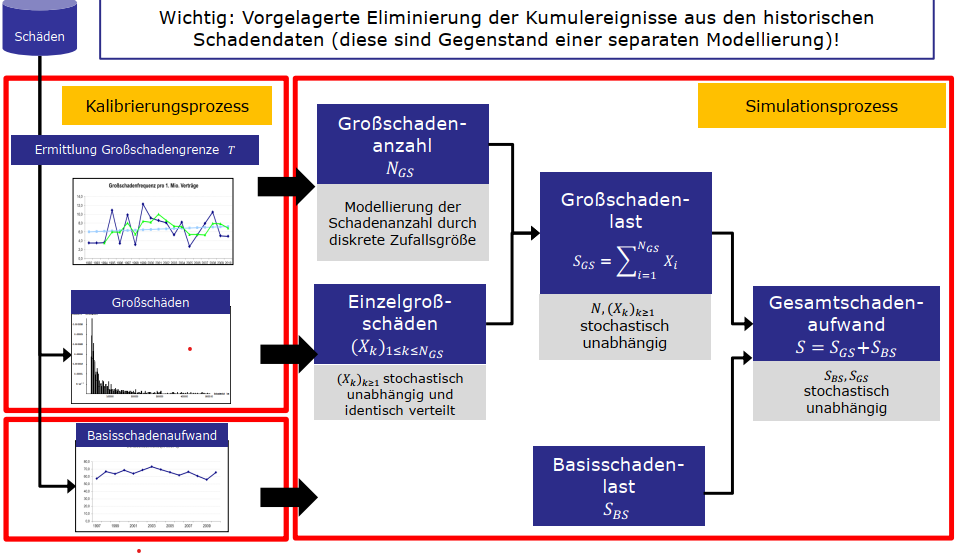
\includegraphics[width= \textwidth]{Bilder/Folie27.png}
\end{figure}

\subsubsection{Kalibrierungsprozess}
\begin{itemize}
\item Abwicklung der Schäaden (Ermittlung voraussichtlicher Endschadenstände)
\item as if-Transformation der Schäden (wenn der Schaden im parametrisierenden Schadenjahr angefallen wäre)
\begin{itemize}
\item Anpassung an aktuelle Bestandsgröße
\item Anpassung an momentanen Geldwert
\item Bereinigung um Trends
\end{itemize}
\item Großschadenfrequenz: Schätze Erwartungswert und Varianz für Frequenz, Anpassung Schadenzahlverteilung (Poisson, Negativ Binomial)
\item Einzelgroßschadenhöhe: Schadenhöhen Anpassung mit schwerer Verteilung: QQ-Plot, Statistische Bewertung
\item Basisschadenlast: Analyse des Schadenbedarfs
\end{itemize}


\section{Modellierung von Katastrophenschäden}

\subsubsection{Definition}
Laut Solvency II stellt das Katastrophenrisiko das Risiko eines außergewöhnlich großen Ereignisses dar – gemäß Rahmenrichtlinie Artikel 105 (2) bezeichnet das Katastrophenrisiko Nicht-Leben das „Risiko eines Verlustes oder einer nachteiligen Veränderung des Werts der Versicherungsverbindlichkeiten, das sich aus einer signifikanten Ungewissheit in Bezug auf die Preisfestlegung und die Annahmen bei der Rückstellungsbildung für extreme oder außergewöhnliche Ereignisse ergibt“.

Beispiel Naturgefahren: Überschwemmung, Hagel, Erdbeben, ... \\
Beispiel Man-Made Gefahren: Explosion, Terror, Cyberangriffe, Luftfahrtunglück

\subsubsection{Analyse und Bewertung des Katastrophenpotentials der versicherten Gefahren}

\begin{itemize}
\item Analyse der Bruttoexponierung (Versicherungssumme, Prämienvolumen,…),
\item Umfang an Rückversicherungsschutz
\item Historische Schäden des Unternehmens, Referenzschäden aus dem Markt
\item Ergebnisse von Quantifizierungsansätzen – Beispiele:
\item Solvency II-Standardformel
\item Externe Modelle
\item Mathematisch-statistische Modellierung
\item Szenarioanalysen
\item Externe (Markt-)einschätzung / Externe Analysen
\item Ergebnis: Qualitative / Quantitative Einschätzung der Materialität jeder Gefahr, Gegenüberstellung mit geeigneter Bezugsgröße des Unternehmens (wie Solvenzkapitalbedarf, Eigenmittel)
\end{itemize}


\subsubsection{Analyse und Bewertung der Datenverfügbarkeit /-qualität}

\begin{itemize}
\item Exposuredaten (Informationen in der benötigten Detailtiefe für den Bestand vorhanden?)
\item Historische Schadendaten
\end{itemize}

\subsection{Charakterisierung von Katastrophenschadenverteilungen}

\begin{itemize}
\item Erwartungswert und Standardabweichung wenig aussagekräftig
\item Daraus folgt: Komplette Verteilungsfunktion benötigt
\item Zwecks Darstellung und Vergleich von Katastrophenschadenverteilungen (auf Jahresbasis) bietet sich die Übersetzung in sog. Überschreitungswahrscheinlichkeiten / Wiederkehrperioden an:
\begin{itemize}
\item Schadenhöhe, die nur in $x\%$ aller Jahre überschritten wird: Ereignis weist eine jährliche Überschreitungswahrscheinlichkeit von $x\%$ auf.
\item Schadenhöhe, die im Mittel nur alle $T$ Jahre beobachtet wird: Ereignis weist die Wiederkehrperiode / Jährlichkeit $T$ auf.
\end{itemize}
\end{itemize}

\subsubsection{Definition}
Bezeichne $N$ die zufällige Anzahl an Ereigniseintritten in einem Jahr und $X_1, ..., X_N$ die zugehörigen Ereignisschadenhöhen sowie\\
$M_N:= max{\{ X_1, ..., X_N\}}$ den max. Ereignisschaden eines Jahres (mit $M_N=0$ für $N=0$)\\
$S:= \sum^N_{i=1} X_i$ den Jahresgesamtschaden \\
Seien weiter $F_{M_N}$ die Verteilungsfunktion von $M_N$ sowie $F_S$ die Verteilungsfunktion von $S$ und $F^{-1}_{M_N}$ und $F^{-1}_S$ihre zugehörigen Inversen. \\
Dann ergeben sind OEP-Kurve und AEP-Kurve als Punktepaare $(T, OEP(T))$ bzw. $(T, AEP(T))$ mit $T \in [1;\infty ]$ und
\begin{equation}
OEP(T) := F^{-1}_{M_N} \left( 1- \frac{1}{T} \right) , AEP(T):= F^{-1}_S \left( 1- \frac{1}{T} \right)
\end{equation}
Die OEP-Kurve stellt den maximalen Ereignisschaden eines Jahres (Maximum Occurrence Loss) in
Abhängigkeit der Wiederkehrperiode dar, die AEP-Kurve wiederum den Jahresgesamtschaden (Annual
Aggregate Loss) \\

Liegen simulierte Ereignisse aus dem Simulationsmodell vor, lassen sich die AEP und OEP-Kurven
aus den empirischen Verteilungen des maximalen jährlichen Ereignisschadens und
Jahresgesamtschadens bestimmen. 

\begin{figure}[ht]
	\centering
	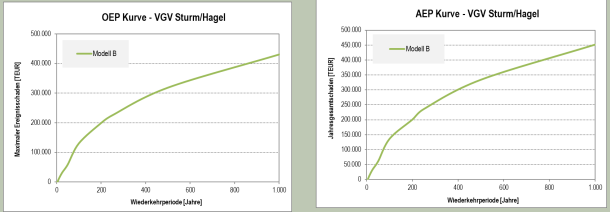
\includegraphics[width= \textwidth]{Bilder/OEPAEP.png}
\end{figure}
 \vspace{4cm}
Für OEP-Kruve ist unter bestimmten Voraussetzung auch analytische Ermittlung möglich:
\begin{figure}[ht]
	\centering
	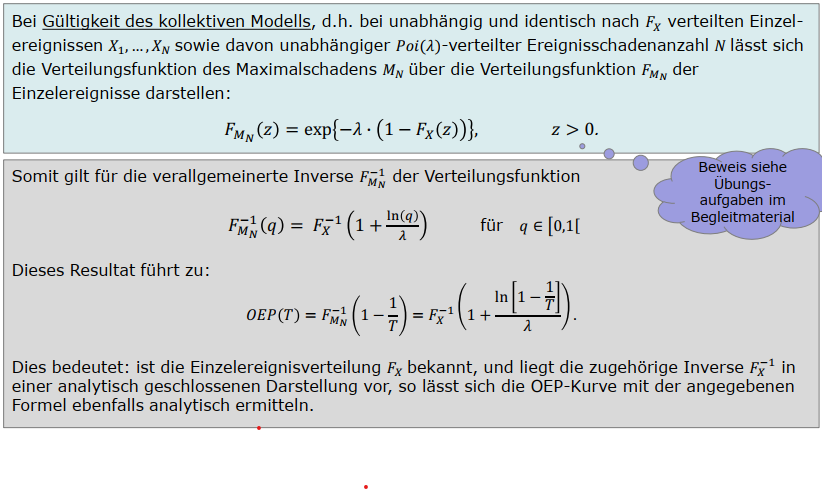
\includegraphics[width= \textwidth]{Bilder/Folie39.png}
\end{figure}

\subsection{Modellierungsansätze für Katastrophenschäden}

\begin{itemize}
\item Mathematisch-statistische Modelle: \\
Schaden wird basierend auf der Schadenerfahrung mit klassischen aktuariellen Verfahren
\item Exposure-basierte probabilitische Modelle: \\
zunächst die schadenbestimmende Ursache eines Ereignisses simulieren und anschließend ihre Schadenwirkungen auf die versicherten Risiken des Unternehmens (Exposure) bestimmt. (Naturgefahrenbereich: geophysikalisch-meteorologische Modelle)
\item Szenario-basierte Modelle: \\
Schadenpotential wird anhand von Szenarioanalysen geschätzt. Schadenhöhe und Eintrittswahrscheinlichkeit bzw. Wiederkehrperiode eines oder mehrerer Einzelszenarien werden mit Hilfe von Verteilungsannahmen in eine Wahrscheinlichkeitsverteilung übersetzt.
\end{itemize}


\subsubsection{mathematisch-statistische (aktuarielle) Modellierung}
Unterteilung in:
\begin{itemize}
\item Explizite Modellierung: im Modell liegt eine eigenständige Katastrophenschadenverteilung für diese Gefahr vor.
\item Implizite Modellierung: keine eigene Katastrophenschadenverteilung, stattdessen: 
\begin{itemize}
\item Die Gefahr wird entweder gemeinsam mit anderen Gefahren modelliert
\item Katastrophenschäden dieser Gefahr werden gemeinsam mit anderen Schadenarten (Basis- oder Großschäden) modelliert
\item Loading: Zuschlag auf Gesamtebene
\end{itemize}
\end{itemize}


\subsection{Explizite Modellierung gemäß mathematisch-statistischer Ansätze}

\subsubsection{Allgemeine Methodik/ Vorgehen}
\begin{itemize}
\item Katastrophenschadenverteilung ergibt sich aus der Anpassung geeigneter Wahrscheinlichkeitsverteilungen an Ereignisschadenhöhen und –anzahlen oder direkt an Jahresschadenlast
\item aus Basis historischer Schadendaten (unternehmenseigene Schadenhistorie) nach as-if Transformation
\end{itemize}

\subsubsection{Mögliche Ansätze/ Beispiele}
\begin{itemize}
\item Ereignisschadenhöhe bedarf in der Regel hinreichend schwerer Verteilung (Bsp: Pareto)
\item Ggf. auch differenziertere, zweistufige Modellierung der Ereignisschadenhöhe
\item Sofern verfügbar: Einbezug von Marktschadendaten
\end{itemize}


\subsection{Implizite Modellierung gemäß mathematisch-statistischer Ansätze}

\subsubsection{Allgemeines Vorgehen}
\begin{itemize}
\item Anpassungen von Wahrscheinlichkeitsverteilungen an die (unternehmenseigenen)
Schadendaten nach as-if Transformation
\item Aber: keine vorgelagerte Trennung der Datengrundlage nach weiteren Einzelgefahren
\item Gemeinsame Kalibrierung von Schäden mehrerer Gefahren, in der Folge keine weitere Unterscheidung nach Gefahr
\end{itemize}

\subsubsection{Mögliche Ansätze/ Beispiele}
\begin{itemize}
\item Naturgefahren: insbesondere für die nicht-materiellen „Nebengefahren“ (Alles außer Sturm, Überschwemmung, Hagel)
\item Manmade: Extrapolation der Großschadenverteilung soll auch Kumulschäden
abdecken
\end{itemize}

\subsubsection{Vorteile}
\begin{itemize}
\item Prinzipiell für alle Arten von Gefahren möglich
\item Transparenz / mehr Freiheitsgrade im Vorgehen
\item Im Wesentlichen statistisches Know-How zur Modellierung notwendig
\end{itemize}

\subsubsection{Herausforderungen} \begin{itemize}
\item Übertragbarkeit der historischen Informationen ggf. fraglich
\item i.a. nur wenige Daten vorhanden, dadurch Kalibrierung unsicher
\item Annahmen über Abhängigkeiten in der Regel grob
\item Schwierigkeit einer adäquaten Extrapolation
\end{itemize}

\subsubsection{Implizite ggü. expliziter Modellierung}
\begin{itemize}
\item Katastrophenschäden weisen äußerst erratisches Verhalten auf, folgen in der Regel anderen Gesetzmäßigkeiten als die Basis- und Großschäden.
\item Andererseits lässt die Datenlage keine atomisierte Modellierung jeder einzelnen Gefahr zu (Fokus der Modellierung auf wirkliche materielle Gefahren)
\end{itemize}

\subsection{Funktionsweise exposure-basierter Modelle}

\subsubsection{1. Portfeuille}
\begin{itemize}
\item Das geophysikalisch-meteorologische Modell benötigt detaillierte Informationen
zum versicherten Portefeuille des Versicherungsunternehmen
\item Der Bestand wird zu einem bestimmten Zeitpunkt abgegriffen, Modell liefert also
streng genommen nur eine Einschätzung zur Gefährdung zum Stichtag des
Bestandsabzugs.
\item Die Validität und Aussagekraft der Modellergebnisse hängt essentiell von der
Qualität der verwendeten Bestandsdaten ab.
\end{itemize}

\subsubsection{2. Ereigniserzeugung}
\begin{itemize}
\item Das Modul umfasst einen Katalog mit historischen und synthetischen Ereignissen,
wobei letztere Ergebnis eines Modellierungs- und Simulationsprozesses sind.
\item Die Intensität der Ereignisse wird anhand schadenbestimmender Parameter
beschrieben, die abhängig von der jeweiligen Naturgefahr sind (Bsp: Windgeschwindigkeit, Hagelkörner, Magnitude)
\end{itemize}

\subsubsection{3. Schadenanfälligkeitsmodul}
\begin{itemize}
\item Die aus dem Ereignis resultierenden Schäden an den versicherten Objekten werden mittels sogenannter Schadenfunktionen ermittelt. Schadenfunktionen beschreiben den funktionalen Zusammenhang zwischen der Intensität eines Ereignisses bzw. der zugehörigen Ausprägungen der Schadenparameter und dem mittleren Schadengrad
\item In den GroundUp-Schäden sind noch keine versicherungsspezifischen Parameter wie
Selbstbehalte oder Limite berücksichtigt
\end{itemize}

\subsubsection{4. Finanzmodel}
\begin{itemize}
\item Im Finanzmodul werden die Vertragsbedingungen und ggf. auch die Rückversicherungsstruktur (Beispiel: Summenexzedent) auf die GroundUp-Schäden angewendet, und so der beim Versicherer tatsächlich verbleibende Brutto- bzw. Nettoschaden ermittelt.
\end{itemize}

Output eines geophysikalischen Modells sind Informationen über die Schadenverteilungen (per
Einzelereignis oder als Jahresaggregat) in komprimierter Form. Eine Event Loss Table (ELT) ist
neben AEP- und OEP-Kurve ein weiterer möglicher Output eines geophysikalischen Modells und
stellt eine Auflistung der im Modell generierten Ereignisse dar.

Geophysikalische Modelle benötigen komplexe Software, daher werden sie nur von großen VU und Rückversicherern betrieben (Externes Modell)


\subsubsection{Event Loss Table (ELT)}
\begin{itemize}
\item Unterscheidet sich nach Anbieter
\item Anbieter AIR:
\begin{itemize}
\item Spalte Year: Simulationsjahr
\item Nr: Index des Ereignisschadens im entsprechenden Simulationsjahr
\item Spalte Company Loss: simulierten Brutto-Schaden des Unternehmens
\item Spalte Event: Ident-Nr. aus Ereigniskatalog
\end{itemize}
\item Anbieter RMS:
\begin{itemize}
\item Spalte EVENTID: Identifizierung
\item Spalte RATE: mittlere Anzahl der Ereigniseintritte in einem Jahr
\item Spalte PERSPVALUE: Erwartungswert der Schadenhöhenverteilung bei Ereigniseintritt
\item die Spalten STDDEVI und STDDEVC: Standardabweichung der Schadenhöhenverteilung bei Ereigniseintritt
\item Spalte EXPVALUE: Obergrenze für den resultierenden Ereignisschaden
\end{itemize}
\item Anbieter CoreLogic:
\begin{itemize}
\item Spalte Event frequency: mittlere Anzahl der Ereigniseintritte in einem Jahr
\item  Spalte Event mean gross loss: Erwartungswert der Schadenhöhenverteilung bei
Ereigniseintritt
\item Spalte Event sigma gross loss: Standabweichung der Schadenhöhenverteilung bei
Ereigniseintritt
\item Event gross limit: Obergrenze für den resultierenden Ereignisschaden
\end{itemize}
\end{itemize}




\subsubsection{Vorteile}
\begin{itemize}
\item Basieren auf multidisziplinärem Know-How
\item Detaillierte Modellierung von Abhängigkeiten
\item Sowohl zur Ermittlung von Wahrscheinlichkeitsverteilungen als auch für (neue) Szenarioanalysen geeignet
\end{itemize}

\subsubsection{Herausforderungen}
\begin{itemize}
\item Sind nicht für alle Gefahren verfügbar
\item Kalibrierung der Modelle (Gefährdung / Vulnerabilitäten) durch den Anbieter vorgegeben, Update der Kalibrierung mit neuer Modellversion
\item Keine komplette Transparenz
\item Für einige Gefahren liegen mitunter gleich mehrere externe Modelle (verschiedener Anbieter) mit unterschiedlichen Modellierungsansätzen vor. 
\end{itemize}

\subsubsection{Eigenentwicklung ggü. externem Modell}
\begin{itemize}
\item Aufwand und Know-How-Bedarf
\item höhere Transparenz
\item mehr Freiheitsgrade bei Modellierung und Kalibrierung
\item Zuschnitt auf unternehmensindividuelle Bedürfnisse
\end{itemize}

\subsection{Modellierung von Katastrophenschäden aus Naturgefahren}

\subsubsection{Beobachtungen aus der Praxis}
\begin{itemize}
\item Durch eingeschränkte Verfügbarkeit einer unternehmenseigenen Schadenhistorie für mathematisch-statistischer Ansätze ist die Modellierung für Sturm, Überschwemmung, Hagel und Erdbeben für deutsche Portefeuilles auf
Basis geophysikalisch-meteorologischer Modelle am weitesten verbreitet
\item Alle weiteren Naturgefahren i.d.R implizit modelliert
\end{itemize}
Teilweise werden im Zuge der Einbindung externer Modelle in das interne Unternehmensmodell noch individuelle Modifikationen am originären Modelloutput vorgenommen (Mischansätze)

\subsection{Modellierung von Man-Made-Katastrophenschäden}

\subsubsection{Beobachtungen aus der Praxis}
\begin{itemize}
\item Die unternehmensindividuelle Schadenhistorie ist i.d.R. limitiert
\item Marktschadenverteilungen für Groß-/Kumulschäden in Man-Made exponierten Sparten sind prinzipiell vorhanden (GDV)
\end{itemize}
Bei den meisten Man-Made Gefahren nutzt man daher die implizite Modellierung oder szenario-basierte Modellierung. In vielen Fällen Rückgriff auf Verteilungen vom Pareto-Typ unter Verwendung, dass es für den
Pareto-Parameter marktweit beobachtbare, spartentypische Ausprägungen gibt.

\subsection{Idealtypischer Modellierungsprozess}

\begin{figure}[ht]
	\centering
	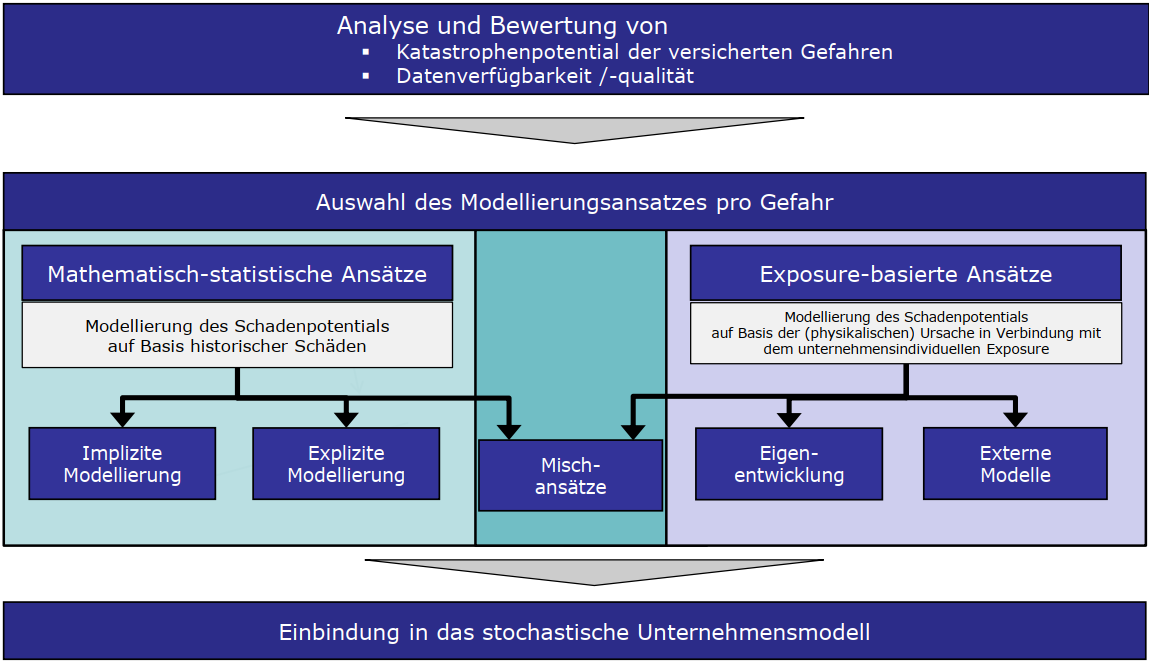
\includegraphics[width= \textwidth]{Bilder/Modellierungsprozess.png}
\end{figure}


\subsection{Einbindung externer (exposure-basierter) Modelle in das interne Modell -
Überblick}

\begin{figure}[ht]
	\centering
	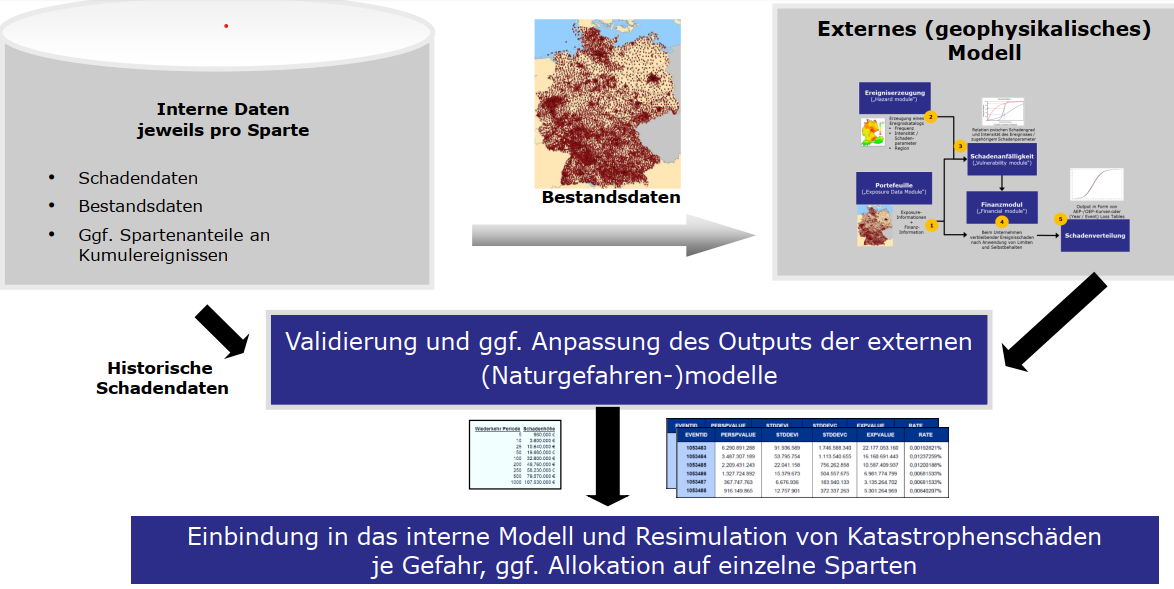
\includegraphics[width= \textwidth]{Bilder/ExternesModell.png}
\end{figure}

\begin{itemize}
\item Die primäre Unsicherheit bezieht sich auf die Unsicherheit über das grundsätzliche Eintreten eines Ereignisses (wird beschrieben durch RATE und PERSPVALUE),
\item die sekundäre Unsicherheit bezieht sich auf die Unsicherheit in der Höhe des
Schadenaufwands bei Eintritt des Ereignisses (wird beschrieben durch die Standardabweichungen)
\end{itemize}


\subsubsection{Actuarial Control Cycle zur Schadenmodellierung}

\begin{figure}[ht]
	\centering
	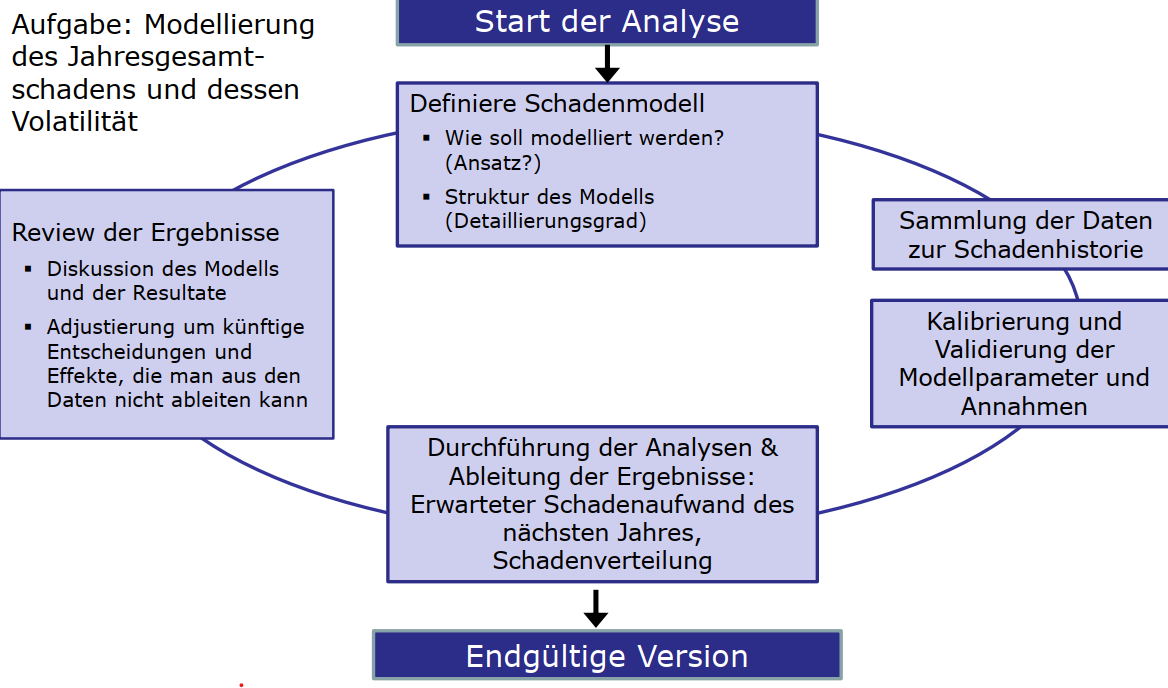
\includegraphics[width= \textwidth]{Bilder/ControlCycle.png}
\end{figure}


\chapter{Rückversicherungsmodellierung}

\subsubsection{Grundidee}

Rückversicherungsanalyse mit stochastischen Unternehmensmodellen:
\begin{itemize}
\item Abbildung von Rückversicherung mithilfe eines internen Modells von zentraler Bedeutung: Einfluss von Rückversicherung hinsichtlich Glättung von Volatilitätsspitzen und Reduktion des Risikokapitalbedarfs
\end{itemize}

\subsubsection{Einsatz interner Modelle zur RV-Analyse}
\begin{itemize}
\item Analyse und Gegenüberstellung der Verteilungen Brutto / Netto bzw. RV-Recoveries ermöglicht genaue Abschätzung von Kosten und Nutzen von RV-Verträgen
\item hilft bei Identifikation von Deckungslücken und der Frage nach der Effizienz der RV
\item  Ableitung unzähliger Kennzahlen möglich (RV-Preis vs. durchschnittliche Recoveries, RV-Preis vs. Risikokapitalersparnis, Gewinnwahrscheinlichkeiten…)
\item Rückversicherungsanalyse mit internen Modellen kann Verhandlungsposition gegenüber Rückversicherern stärken
\item Vor Solvency II für viele VU Motivation zum Aufbau interner Modelle, heute oft zum
Nachweis des „Use Test“ (Verwendungstests) unter Solvency II verwendet
\end{itemize}

\chapter{Stochastische Modellierung des Reserverisikos und Erzeugung von Cashflows}

\section{Modellierung des Reserverisikos und Generierung von Cashflows}
\begin{figure}[ht]
	\centering
	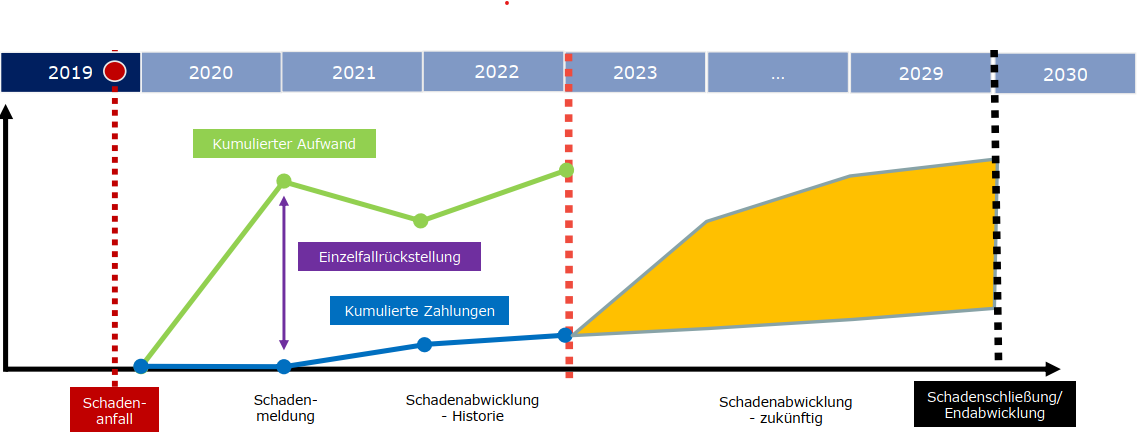
\includegraphics[width= \textwidth]{Bilder/Einzelschaden.png}
\end{figure}
Aktuarielle Reservierungsverfahren liefern mit dem Best-Estimate für die Schadenrückstellungen eine Punktschätzung („wahrscheinlichkeitsgewichtetes Mittel“) und damit lediglich ein mögliches Auskommen der Reserve

\begin{itemize}
\item Das Reserverisiko beschreibt allgemein die Unsicherheit, die mit der Vorhersage der Abwicklung bereits eingetretener Schäden verbunden ist (zur genauen Definition kommen wir später).
\item Das Reserverisiko beinhaltet zwei Aspekte:
\begin{itemize}
\item Höhe der Reserven (Reservierungsrisiko (= Unsicherheit über die zukünftige Auszahlungshöhe)
\item Auszahlungszeitpunkte der Zahlungen („Abwicklungsmuster“) (Auszahlungsrisiko (= Unsicherheit über die konkreten Auszahlungszeitpunkte))
\end{itemize}

\end{itemize}

\subsection{Stochastische Modelle für die Schadenabwicklung}

\begin{figure}[ht]
	\centering
	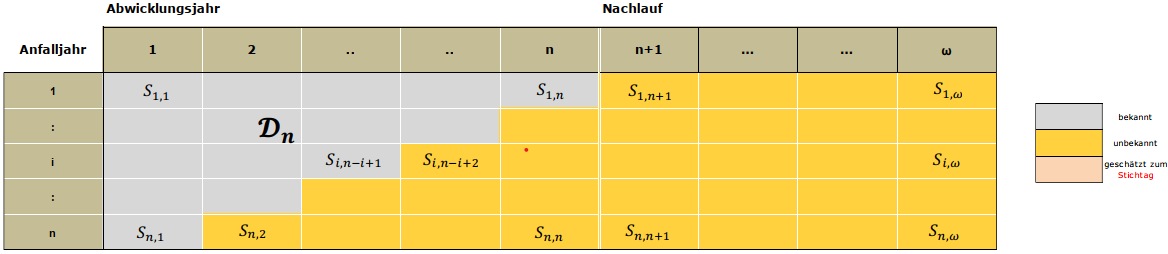
\includegraphics[width= \textwidth]{Bilder/Dreieck.png}
\end{figure}

\subsubsection{Ausgangsituation/ Notation}
\begin{itemize}
\item $S_{i,k}$ bezeichnet die (nominalen) inkrementellen Zahlungen für das Anfalljahr $1 \leq i \leq n$ im Abwicklungsjahr $1 \leq k \leq \omega$ (mit $\omega$ Endabwicklungszeitpunkt)
\item $C_{i,k} = \sum^k_{j=1} S_{i,j}$ repräsentiert die kumulierten Zahlungen eines Anfalljahres nach $k$ Abwicklungsjahren
\item Das Schadendreieck $D_n:= \{S_{i,k} \}_{i+k\leq n+1}$ enthält die bis $T=n$ bereits geleisteten Schadenzahlungen
\item Die Zahlungen $\{S_{i,k}\} _{1\leq i \leq n, n-i+1 < k \leq \omega}$ sind zum Zeitpunkt $T=n$ noch unbekannt und damit ebenfalls:
\begin{itemize}
\item die nominale Bedarfsreserve $R^{(n)}_i := \sum^\omega_{k=n-i+2}S_{i,k}$ eines einzelnen Anfallsjahres $1\leq i \leq n$
\item die nominale Bedarfsreserve $R^{(n)} := \sum^n_{i=1} R_i^{(n)}$ aller Anfalljahre
\item der nominale Endschadenaufwand ("Ultimate") $U_i:=C_{i,\omega}$ eines Anfalljahres $1\leq i \leq n$
\end{itemize}
\end{itemize}

\begin{figure}[ht]
	\centering
	\includegraphics[width= \textwidth]{Bilder/Schätzprozess.png}
\end{figure}

Zur Messung des Reserverisikos ist unabhängig vom konkreten Risikohorizont die Formulierung eines geeigneten stochastischen Modells für die Schadenabwicklung notwendig, welches konsistent zum  verwendeten Reservierungsverfahren $\mathcal{T}_n$ für die Best-Estimate Schätzung ist.

\begin{figure}[ht]
	\centering
	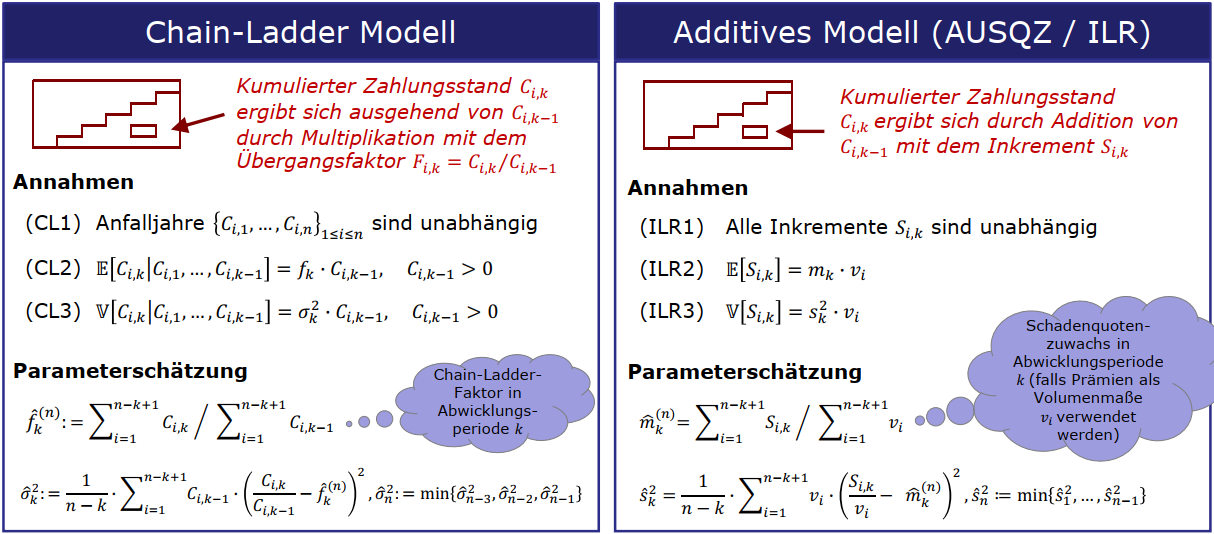
\includegraphics[width= \textwidth]{Bilder/Modelle.png}
\end{figure}


\subsubsection{Definition ultimatives Reserverisiko}
Als ultimatives Reserverisiko wird das Risiko bezeichnet, dass die Best-Estimate
Rückstellungen für angefallene, aber noch nicht abgewickelte Versicherungsfälle nicht
ausreichen, um allen zukünftigen Schadenzahlungen bis zur vollständigen Abwicklung
nachzukommen.

Maßgebliche Größen für die Messung sind die Abweichungen der zukünftigen Zahlungen von den zugehörigen Reserveschätzern:
\begin{itemize}
\item Einzelnes Anfalljahr $1 \leq i \leq n$: $R^{(n)}_i - \hat{R}^{(n)}_i= U_i - \hat{U}^{(n)}_i$
\item Gesamtportfolio, d.h. alle Anfalljahre $\{1,...,n\}$: $R^{(n)} - \hat{R}^{(n)} = \sum^n_{i=1} (R^{(n)}_i - \hat{R}^{(n)}_i)$
\end{itemize}


\subsection{Ansätze zur Quantifizierung des ultimativen Reserverisikos}

\begin{figure}[ht]
	\centering
	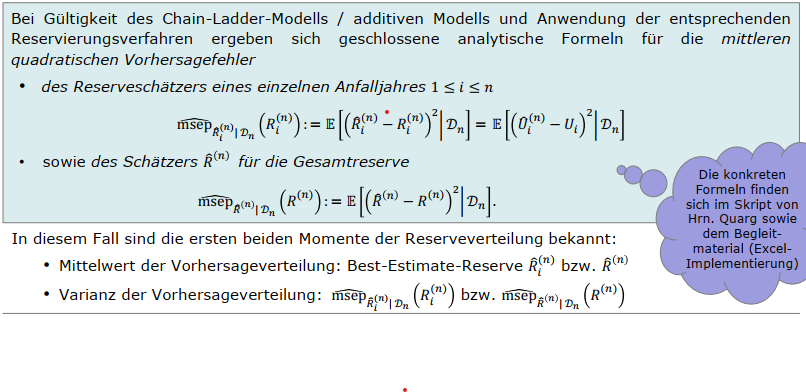
\includegraphics[width= \textwidth]{Bilder/Schaetzer.png}
\end{figure}

Wahl der Reserveverteilung für das ultimative Reserverisiko:
\begin{itemize}
\item lediglich zweiparametrige Verteilungen 
\item  Die Lognormal- und Gammaverteilung zeichnen sich durch ihre Rechtsschiefe aus, die Lognormalverteilung hat dabei in der Regel den schwereren Tail.
\item Einschränkungen der Normalverteilung: symmetrisch, kein ausschließlich positiver
Wertebereich
\end{itemize}

\begin{figure}[ht]
	\centering
	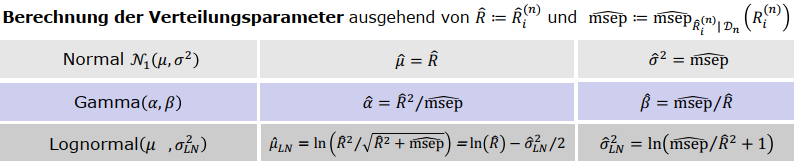
\includegraphics[width= \textwidth]{Bilder/Verteilungsparameter.png}
\end{figure}

\begin{figure}
	\centering
	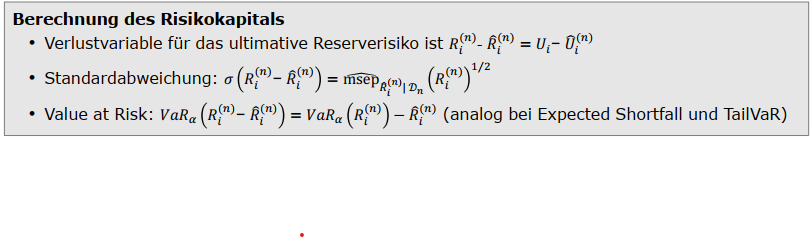
\includegraphics[width= \textwidth]{Bilder/Risikokapital.png}
\end{figure}

\vspace{1cm}
Mögliches Vorgehen:
\begin{itemize}
\item Simuliere anhand der mittleren quadratischen Vorhersagefehler (gegeben die Dreieckshistorie $D_n$) die Bedarfsreserven pro einzelnem Anfalljahr aus einer parametrischen Wahrscheinlichkeitsverteilung
\item Da die Vorhersagen der Reserven für die einzelnen Anfalljahre weder unabhängig (gemeinsamer
Schätzprozess) noch vollständig positiv (Unabhängigkeit im Prozess) korreliert sind, sind Einzelreserven geeignet in Abhängigkeit zu bringen, damit der Vorhersagefehler der Gesamtreserve nach Aggregation der Einzelreserven reproduziert wird.
\item Aus den analytischen Formeln zu den Vorhersagefehlern lassen sich zusätzlich lineare Korrelationen ermitteln, die zur Kalibrierung der Abhängigkeiten genutzt werden können.
\end{itemize} 

In den wenigsten Fällen: Verwendung von Basisverfahren für Best-Estimate-Schätzungen \\
Stattdessen: Variationen des Basisverfahrens (Ausschluss einzelner Übergangsfaktoren, Beschränkung der Übergangfaktoren, Glättung der Chain-Ladder-Faktoren)

\subsubsection{Wie ist bei der Risikobewertung mit Modifikationen der
Basisverfahren umzugehen?}
\begin{itemize}
\item Grundsätzlich: Modifikationen können schwankungserhöhend, aber auch
schwankungsmindernd wirken
\item Pragmatischer Ansatz: Übertrage den theoretischen Vorhersagefehler
unter dem Basisverfahren bzw. dem zugehörigen stochastischen
Abwicklungsmodell (sofern analytisch ermittelbar) auf die mit dem Verfahren $\mathcal{T}_n$ tatsächlich geschätzte Best-Estimate-Reserve
\item Zur Sicherstellung größtmöglicher Konsistenz zwischen Best-EstimateBewertung und Risikomessung sollte das Basisverfahren hinreichend nahe
an $\mathcal{T}_n$ liegen
\end{itemize}

Bei Schwierigkeiten: Bootstrapping-Verfahren


\chapter{Überleitung in die einjährige Risikosicht in der Versicherungstechnik}

\subsection{Allgemeine Überlegungen zum einjährigen Risikohorizont}
Das SCR (Solvenzkapitalanforderung) entspricht dem Value-at-Risk der Veränderung der
Basiseigenmittel eines Versicherungs- oder Rückversicherungsunternehmens zu einem
Konfidenzniveau von 99,5 % über den Zeitraum eines Jahres.

\begin{figure}[ht]
	\centering
	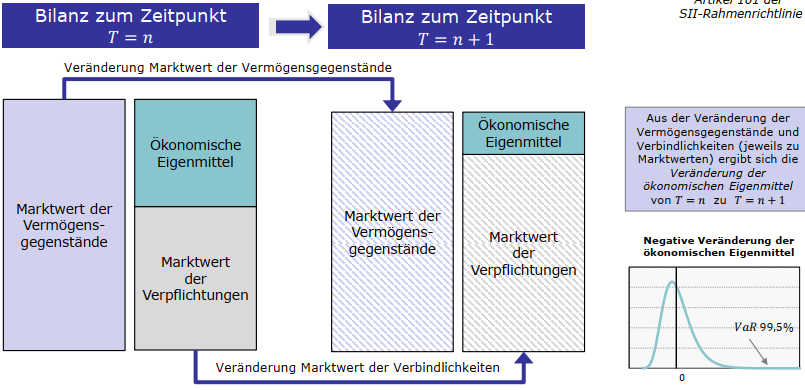
\includegraphics[width= \textwidth]{Bilder/SCR.png}
\end{figure}

\begin{figure}[ht]
	\centering
	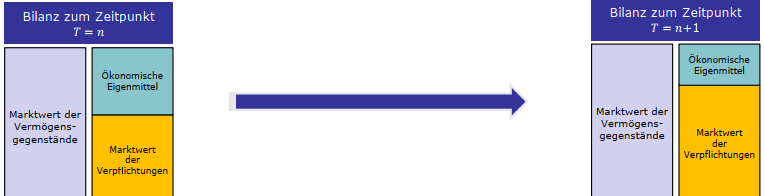
\includegraphics[width= \textwidth]{Bilder/Risikohorizont.png}
\end{figure}



Zu Beginn des Kalenderjahres (erstes Rechteck):
\begin{itemize}
\item liegt eine ökonomische Bewertung der vt. Verbindlichkeiten zum Stichtag $T=n$ vor
\item Bester Schätzwert ist brutto (ohne Abzug von RV-Verträgen)
\item Einforderbare Beträge werden gesondert berechnet
\end{itemize}



Während des Kalenderjahres (Pfeil):
\begin{itemize}
\item werden Schäden aus Altjahren gemeldet, bezahlt, Schadenrückstellungen aufgelöst und neu gebildet
\item fallen Kosten für den Versicherungsbetrieb und Schadenregulierung an
\item Angefallene Schäden im Kalenderjahr gemeldet,  bezahlt, Schadenrückstellungen  gebildet
\end{itemize}


Am Ende des Kalenderjahres (Zweites Rechteck)
\begin{itemize}
\item erfolgt ökonomische Neubewertung der vt. Verbindlichkeiten zum Stichtag ($T=n+1$) unter der Berücksichtigung der Entwicklungen
\end{itemize}

\begin{itemize}
\item In der einjährigen Risikosicht werden die Auswirkungen von Eintritt und Abwicklung der Schäden auf die ökonomischen Eigenmittel innerhalb des auf den Bewertungsstichtag folgenden Kalenderjahres betrachtet.
\item Die Trennung zwischen Prämien- und Reserverisiko erfolgt anhand des Zeitpunkts des Schadenanfalls (beim Reserverisiko werden ausschließlich die bis zum Bewertungsstichtag bereits angefallenen Schäden betrachtet, beim Prämienrisiko die nach dem Bewertungsstichtag anfallenden Schäden).
\end{itemize}

\begin{figure}[ht]
	\centering
	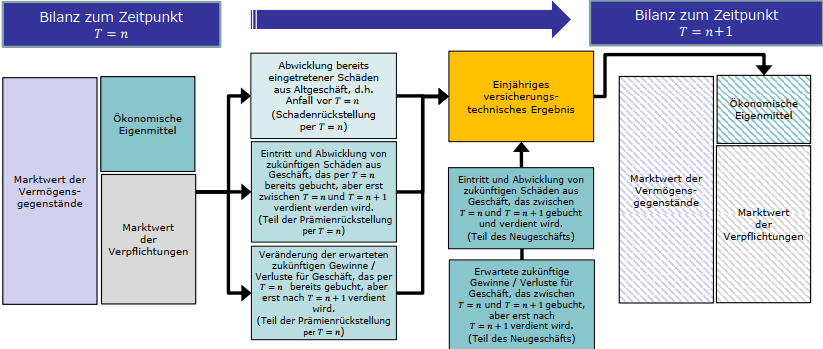
\includegraphics[width= \textwidth]{Bilder/Kalendersicht2.png}
\end{figure}


Vt. Ergebnis des nächsten Kalenderjahres setzt sich zusammen aus:
\begin{itemize}
\item Zukünftige Gewinne/Verluste aus der Abwicklung der Altschäden (aus
Anfalljahren $1, …, n$) während des nächsten Kalenderjahres
\item Zukünftige Gewinne/Verlusten aus Anfall und Abwicklung von Neuschäden aus
zukünftig verdientem Geschäft (Anfalljahr $n+1$) während des nächsten
Kalenderjahres
\end{itemize}


\subsection{Der einjährige Risikohorizont im Reserverisiko}
\begin{figure}[ht]
	\centering
	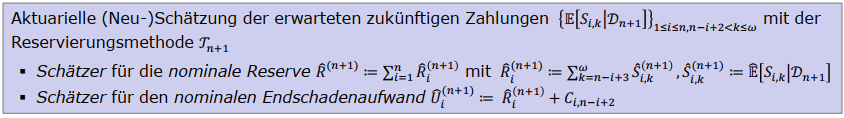
\includegraphics[width= \textwidth]{Bilder/Schaetzer2.png}
\end{figure}

\begin{figure}[ht]
	\centering
	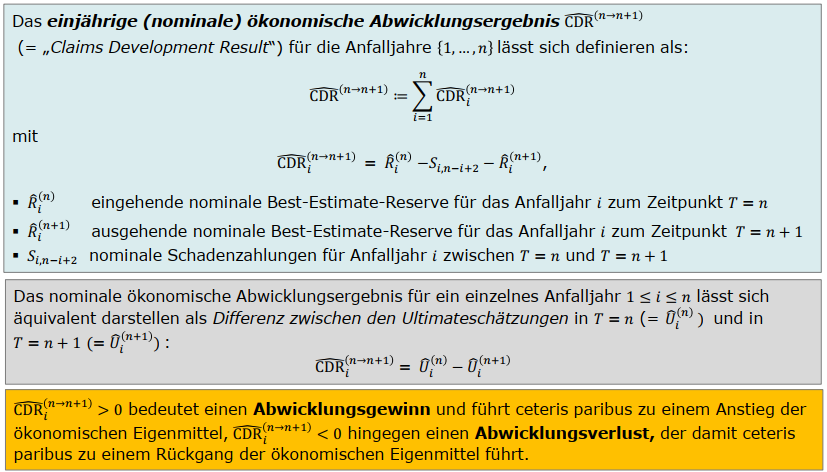
\includegraphics[width= \textwidth]{Bilder/AbwErg.png}
\end{figure}

\subsubsection{Definition}
Als einjähriges (nominales) Reserverisiko wird das Risiko eines (nominalen)
Definition ökonomischen Abwicklungsverlustes über den Zeitraum von einem Kalenderjahr bezeichnet.

\subsubsection{Ziel}
Modellierung der kompletten Vorhersageverteilung des einjährigen nominalen ökonomischen Ziel Abwicklungsergebnisses $\hat{CDR}^{(n\rightarrow n+1)}$ gegeben die Dreieckshistorie $D_n$.

\subsection{Direkte Anpassung der CDR-Verteilung gemäß Analytik}








\end{document}